\documentclass[a4paper,10pt]{article}

%Packages
\usepackage{graphicx}
\usepackage{grffile}
\usepackage{color}
\usepackage{float}
\usepackage[utf8]{inputenc}

\author{Illusion Solutions}

%Document start
\begin{document}
	
	%Title Page
	\begin{titlepage}
		\begin{center}
			\line(1,0){300} \\
			[0.1cm]
			\textsc{\Huge
				PowerCloud\\
				Instruction Manual
			} \\
			\line(1,0){300} \\
			[2.0cm]
			\textsc{\Large
				Illusion Solutions
			} \\
			[3.5cm]
			
		\end{center}
		\begin{flushright}
			\textsc{\Large
				Stuart Andrews\\ 
				12153983\\
				Marc Antel\\
				12026973\\
				Mothusi Masibi\\
				12004589\\
				Brandon Wardley\\
				29005150\\
				[4.0cm]
			}
		\end{flushright}
		\begin{center}
			\today
		\end{center}
	\end{titlepage}
	
	\newpage
	\tableofcontents
	\thispagestyle{empty}
	\newpage
	
	\section{Overview}
	The goal of this project will be to measure the power consumption of machines
	in easy, cost effective way backed by a powerful cloud based interface. Which
	will allow the client to interrogate the data in a meaningful way. Providing in
	depth knowledge of the power consumption. This will allow them to reduce
	costs and save power leading to our ultimate goal of creating a better world
	for tomorrow. There is two main components to the project. There will be
	the software that runs on the particle(Electronic device) and is responsible for
	logging data to the server. Then the web application that will be responsible
	for displaying the power consumption. Advanced mathematical analysis and
	manipulation will be performed on the data. The project will have an optional
	goal of performing analysis on harmonics. All electronic equipment required
	will be provided to the students.

	\section{System Configuration}
	The system is comprised of multiple components, a web application and a Java-MQTT server, with Google's Firebase as the persistence.
	\begin{itemize}
		\item a power usage device,
			\begin{itemize}
				\item The device consists of multiple separate parts:
				\begin{itemize}
				\item A Particle Photon
					\begin{itemize}		
						\item Uses header pins connected to a bread board to read values.
						\item Uses the MQTT messaging protocol to send data to the Java server on port 1883.
						\item Uses the Particle API for everything else.
						\item The Particle code is C++.
					\end{itemize}
				\item A multifunction power monitor, used to measure kWh.
				\item A current transformer, used to acquire accurate and real time current.
				\item A relay to control the flow of electricity through the device.
				\item A trip switch to manually turn the device on or off.
				\end{itemize}					
			\end{itemize}		
		\item a Java-MQTT server,
			\begin{itemize}		
				\item Uses the Moquette MQTT library to listen, on port 1883, for messages sent from the Device.
				\item Uses the Firebase API in order to send and retrieve data, via HTTPS, to and from the database.
			\end{itemize}				
		\item a web application,
			\begin{itemize}		
				\item Uses AngularJS.
				\item Uses the Firebase API in order to send and retrieve data, via HTTPS, to and from the database.
			\end{itemize}				
		\item Google Firebase
			\begin{itemize}
				\item Uses HTTPS to communicate with the Java server and the Web application.
			\end{itemize}
	\end{itemize}
	\section{Compiling and Installing from Source Code}
	\subsection{Pre-requisites}
	\textbf{Software}
	Before proceeding please ensure you have the following software installed on your system:
	\begin{itemize}
		\item NodeJS and NPM
		\item Bower
		\item Gulp
		\item Particle Dev
		\item Java 8
		\item Maven
	\end{itemize}
	
	\textbf{Hardware}
	\begin{itemize}
		\item A Particle Photon.
		\item A computer with internet access which does not block incoming and outgoing connections on port 1883 and 80.
	\end{itemize}
	
	\subsection{Firmware}
		\subsubsection{Manual Particle Photon Setup}
			Compile and flash the photon with the following commands, please take note 
			that if you run the application server on a local machine, retrieve the IP 
			address and insert it into the firmware's code as shown below.\\
	
			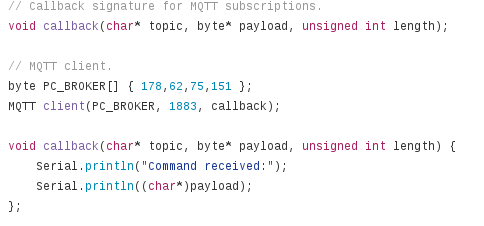
\includegraphics[scale=0.5]{images/firmware.png}
	
	
			Follow the instructions here in order to compile the firmware using Particle 
			Dev.
			\\
			\begin{itemize}
				\item Open the firmware using Particle Dev.
				\item Click on "\textit{Compile using Partcicle Cloud}".
				\item Select the device to flash.
				\item Click on "\textit{flash device}".
			\end{itemize}
			
			\textit{If you run into errors, please see the troubleshooting guide at the end of this document.}
		\subsubsection{How to Register Device Onto System}
			In order to register a new device onto the PowerCloud system, follow the steps:
			
			\begin{itemize}
				\item Login to https://power-cloud.tech.
				\item Proceed to the profile tab, and click on it.
				\item Once in the profile tab (see page x, picture y) locate Particle.io Settings.
				\item Using your Particle login details, login into Particle.io to gain access to the Particle API.
				\item Now locate Devices on the left hand side, click on it.
				\item Locate the Add Device tab, click "\textit{New}".
				\item Do the following:
				\begin{itemize}
					\item Enter the name of the device e.g. "PhotonIT444".
					\item Enter the appliance that which the device is attached e.g. "IT 4-44".
					\item Enter the ID of the Photon, in order to claim it to your Particle account.
					\item Enter the threshold of the device, so as to protect your device from potentially high currents that could prove disastrous should they reach the appliance.
					\item Select the time interval between readings from the drop down list.
				\end{itemize}
			\end{itemize}
		\subsubsection{How to Register on the Particle.io Site}
			\begin{itemize}
				\item Navigate to https://login.particle.io/console.
				\item Click "\textit{Sign Up}".
				\item Enter the ID of the Photon, in order to claim it to your Particle account.
				\item Do the following:
				\begin{itemize}
					\item Enter an email for your username.
					\item Enter a password and verify it.
					\item Click sign up.
				\end{itemize}
			\end{itemize}
				
	\subsection{Application Server}
	Currently, the \textit{application-server} branch hosts the source code for 
	the Application Server. It needs to be compiled using maven and run on a 
	device which doesn't block incoming and outgoing connections on port 1883.\\
	
	\textbf{Compiling the Application Server}\\
	Download the sources from GitHub and compile:\\
	
	\begin{itemize}
		\item \textit{\$ mvn package}
	\end{itemize}		
	
	\textit{If you run into errors, please see the troubleshooting guide at the end of this document.}
	
	\newpage
	\section{Starting PowerCloud}
	\subsection{Firmware}
	Once the firmware has been compiled and the binary file produced. Flash the photon with the following command:
	
	\begin{itemize}
		\item \textit{particle serial flash Photon Name *.ino}
	\end{itemize}
	
	\subsection{Application Server}
	Once the application server has been compiled, change your directory to IllusionSolutions/test/, run the application server using the following command
	
	\begin{itemize}
		\item \textit{java -jar applicationServer-*.jar}
	\end{itemize}
	
	\subsection{Web Application}
	To start the PowerCloud Web application open the console.
	
	\begin{itemize}
		\item \textit{npm install}
		\item \textit{bower install}
		\item \textit{gulp serve}
	\end{itemize}
	
	The web application should now be available on \textbf{http://localhost:9000/}
	
	\begin{figure}[H]
		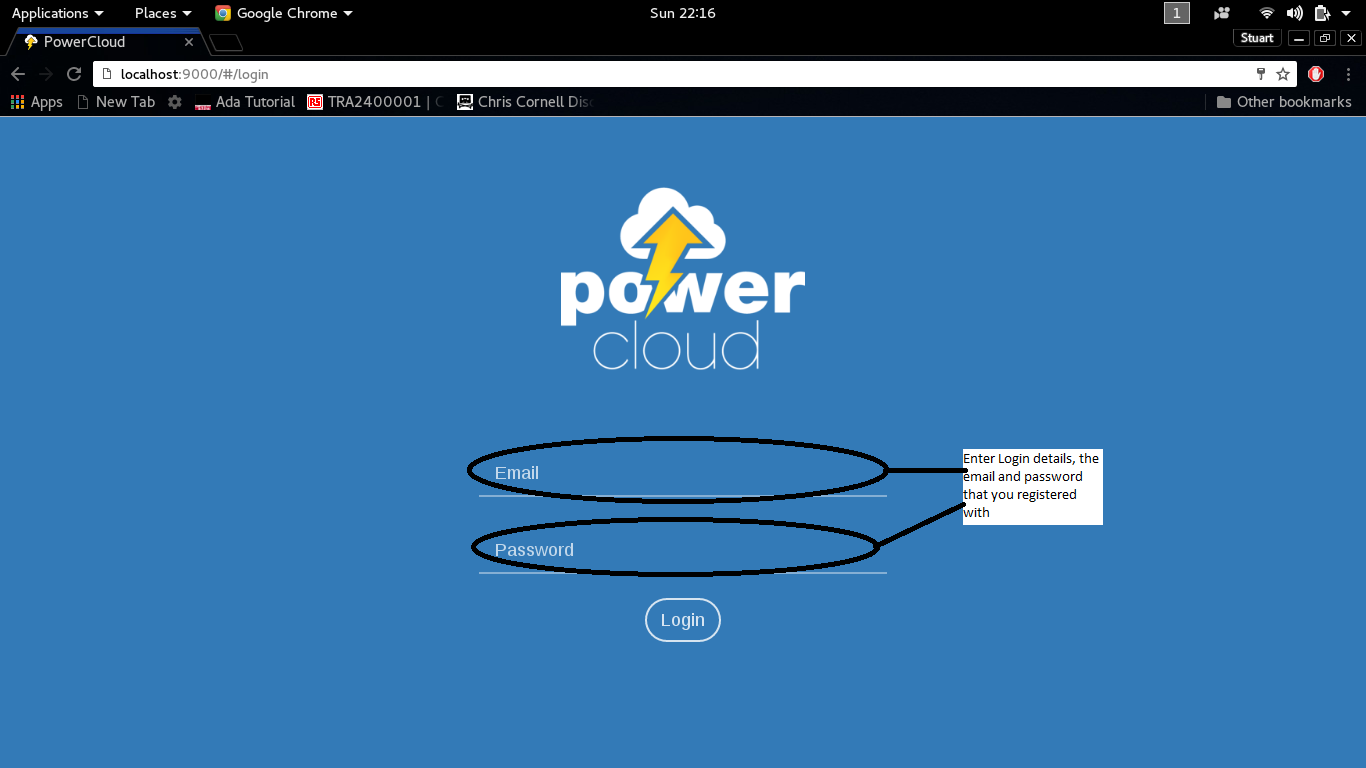
\includegraphics[width=\textwidth]{images/login.png}
		\caption{Initial login screen. \label{overflow}}
	\end{figure}
	
	\begin{figure}[H]
		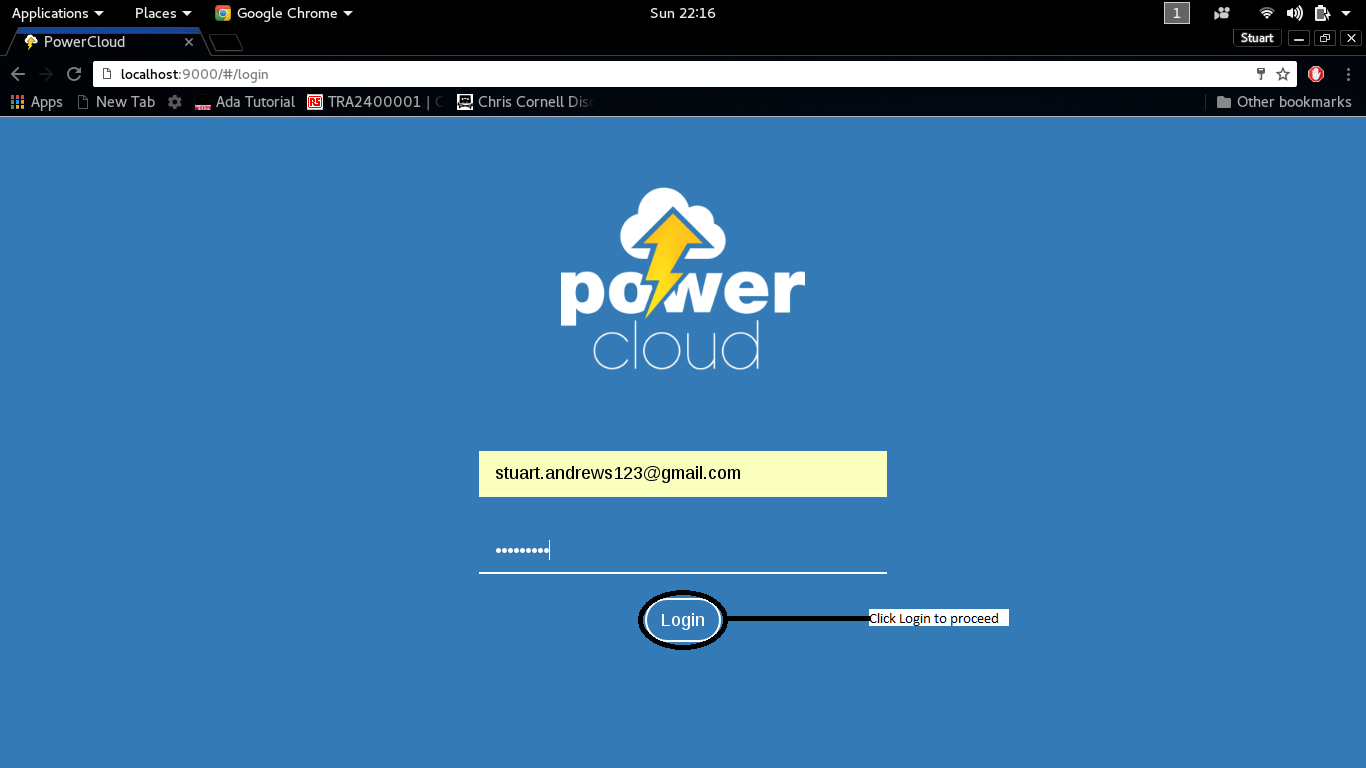
\includegraphics[width=\textwidth]{images/login2.png}
		\caption{Completed login screen. \label{overflow}}
	\end{figure}
	
	\begin{figure}[H]
		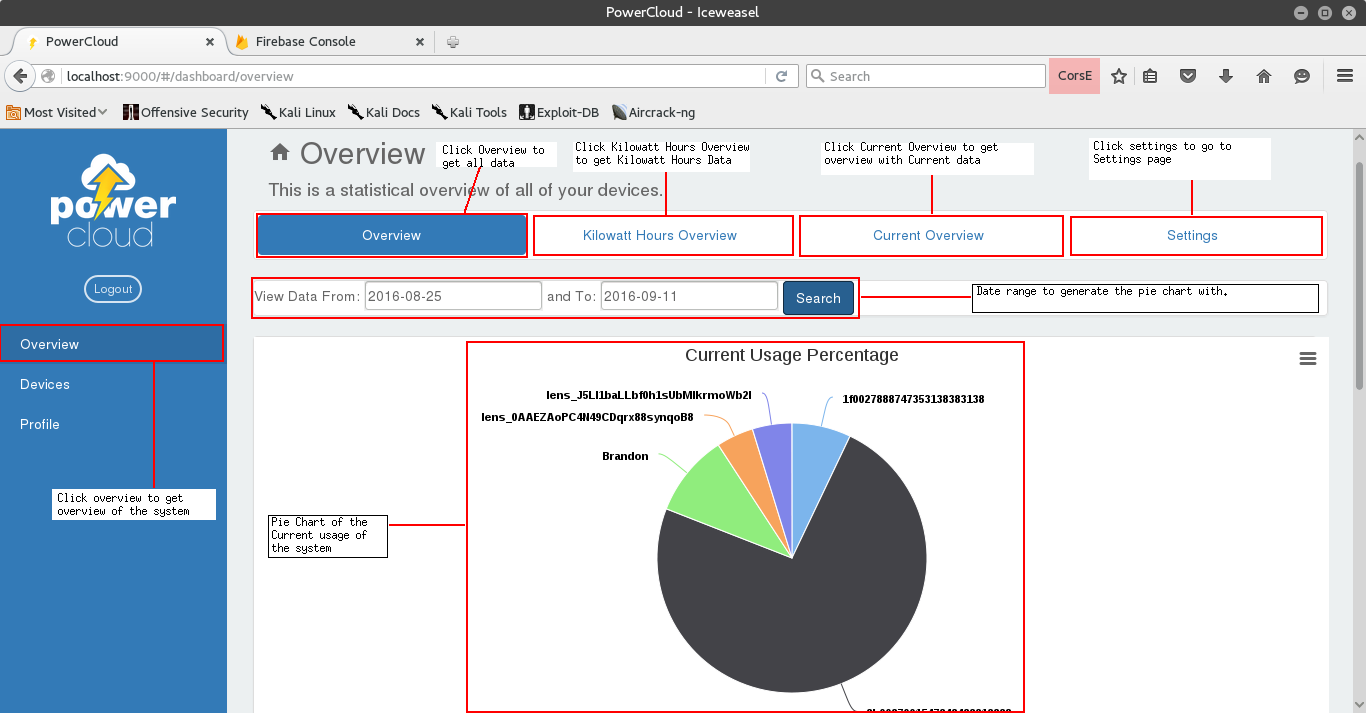
\includegraphics[width=\textwidth]{images/Overview.png}
		\caption{Overview screen. \label{overflow}}
	\end{figure}
	
	\begin{figure}[H]
		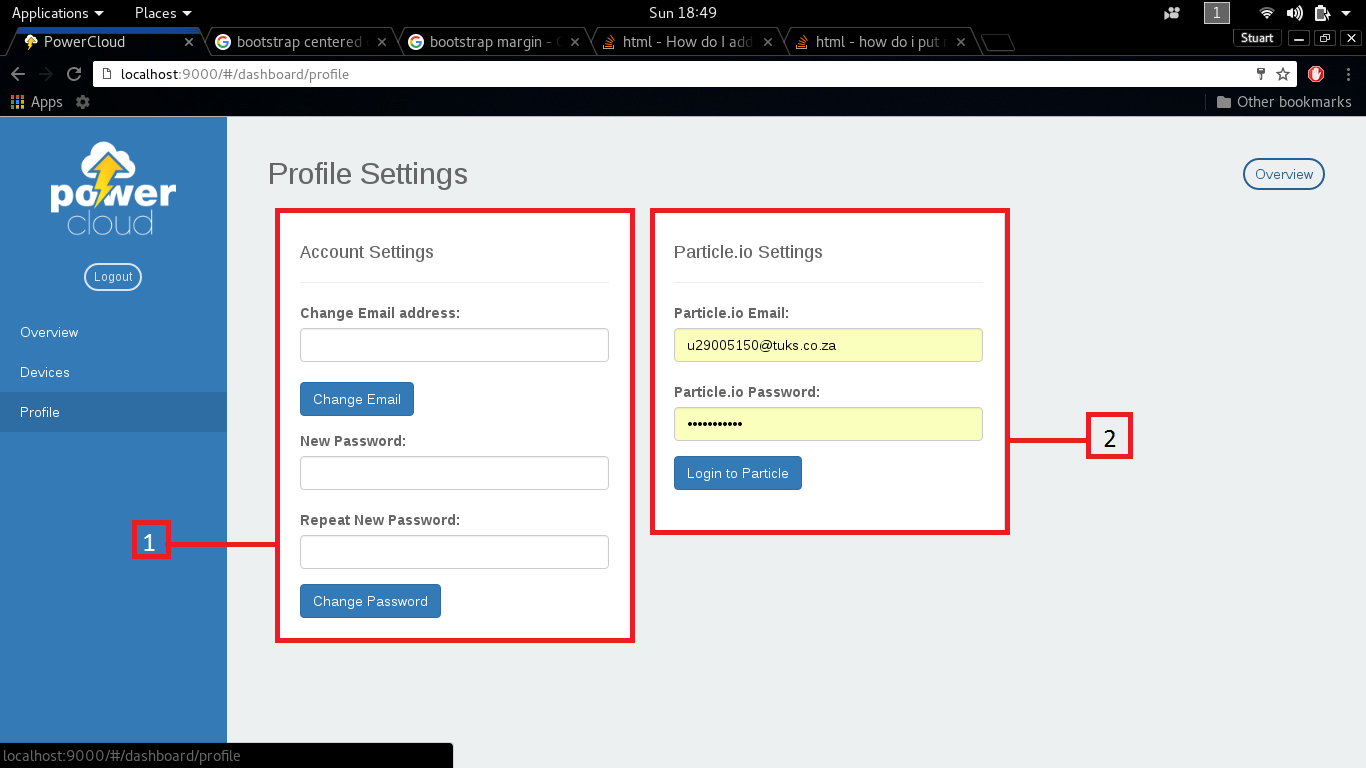
\includegraphics[width=\textwidth]{images/profile.png}
		\caption{Profile settings. \label{overflow}}
	\end{figure}
	
	\begin{figure}[H]
		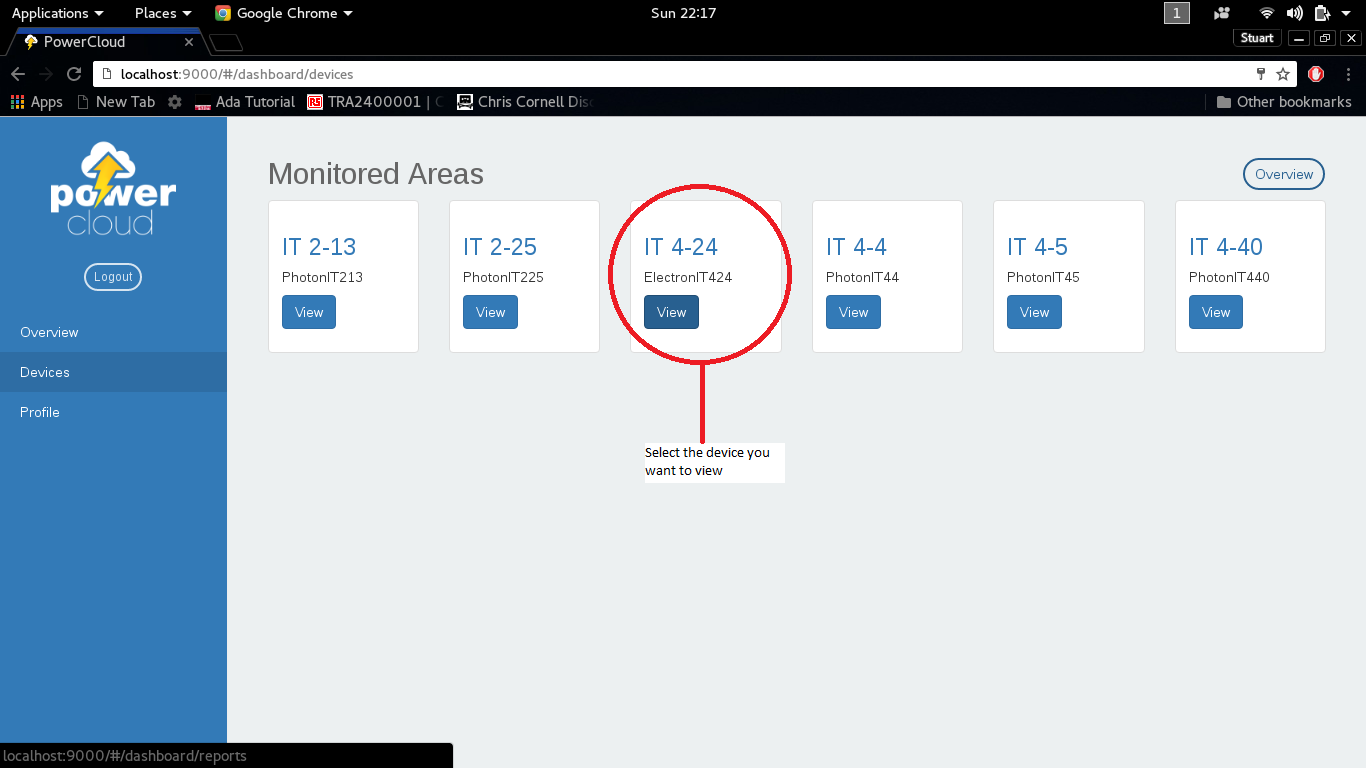
\includegraphics[width=\textwidth]{images/view.png}
		\caption{Monitored Areas. \label{overflow}}
	\end{figure}
	
	\begin{figure}[H]
		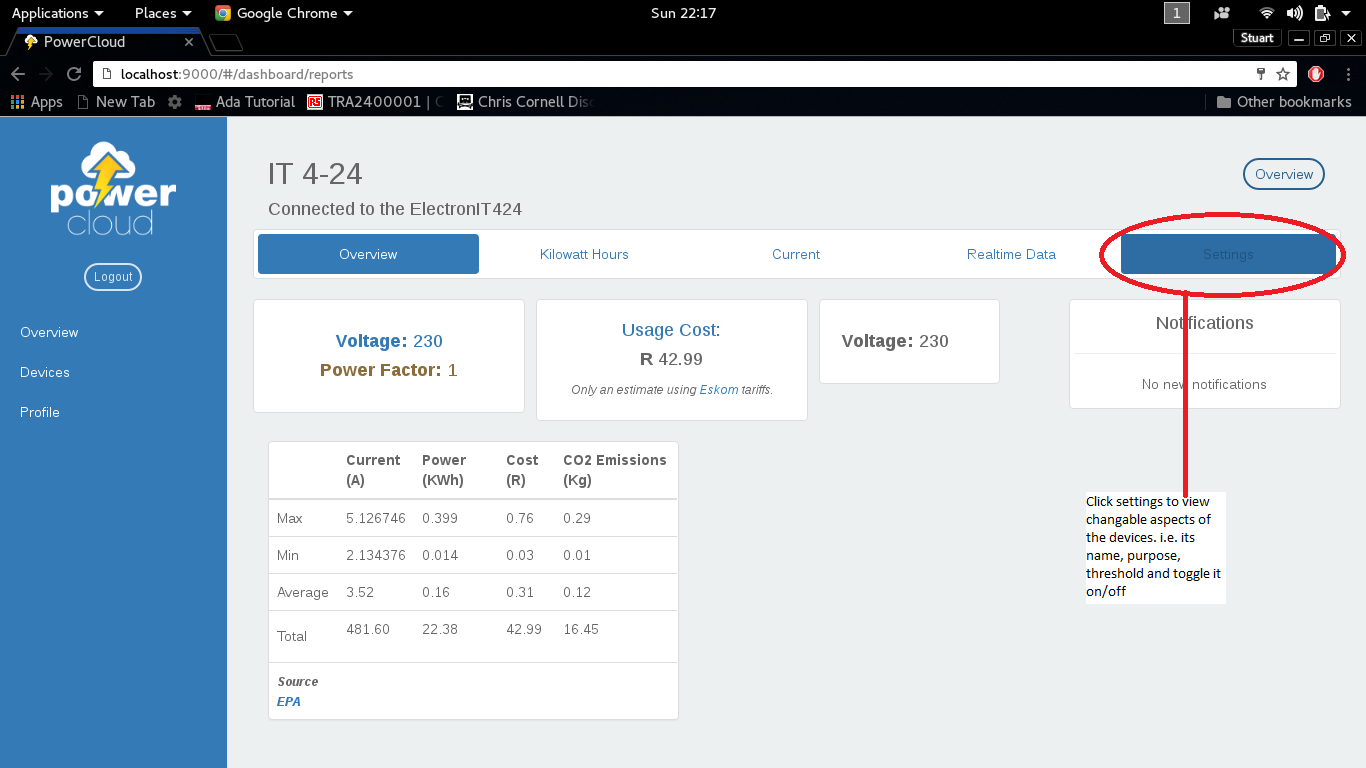
\includegraphics[width=\textwidth]{images/settings1.png}
		\caption{Data display page. \label{overflow}}
	\end{figure}
	
	\begin{figure}[H]
		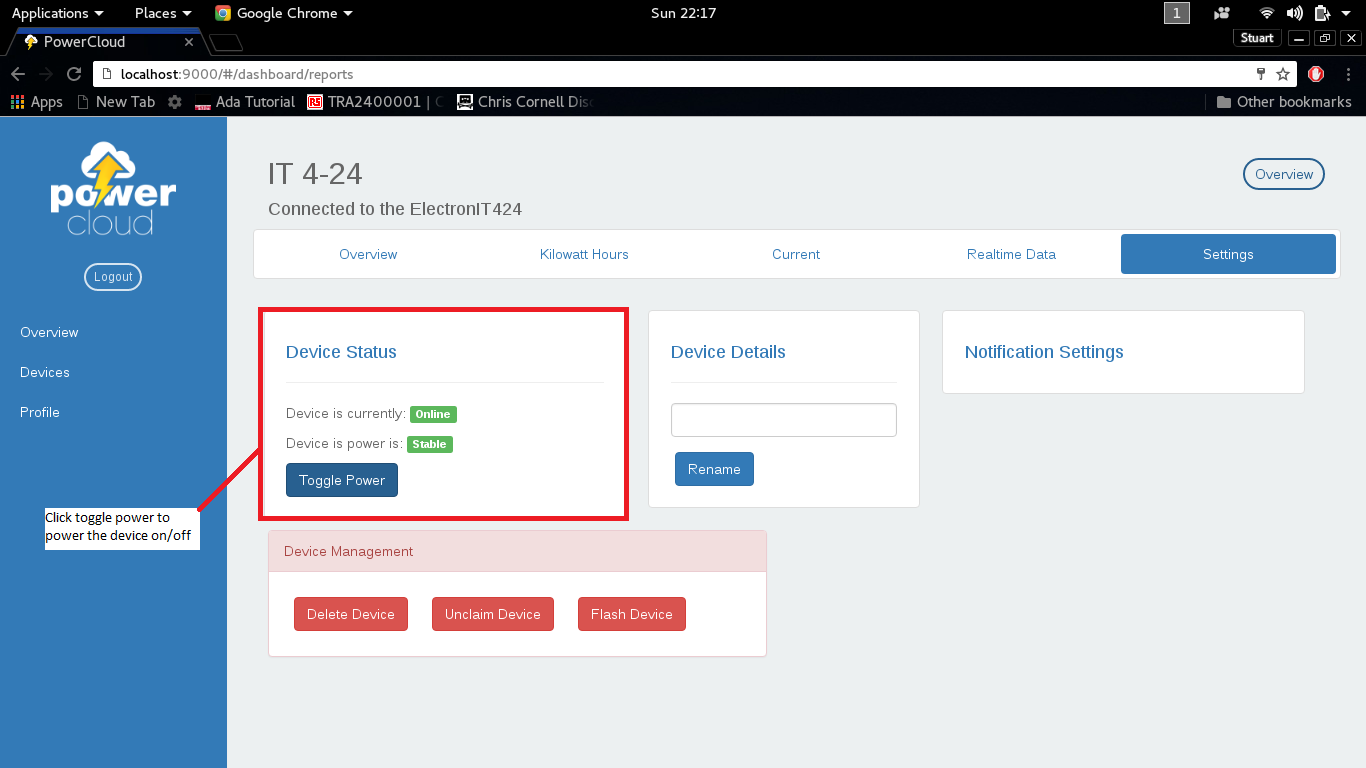
\includegraphics[width=\textwidth]{images/settings.png}
		\caption{Device settings page. \label{overflow}}
	\end{figure}
	
	\newpage
	\section{Troubleshooting}
	\textbf{I am getting errors when trying to install through the console.}
	\begin{itemize}
		\item Try using sudo before the command. Example: sudo npm install particle-cli
	\end{itemize}
	
	\textbf{The Web Application won't run and is giving errors when executing the gulp serve command.} 
	\begin{itemize}
		\item Make sure you've run npm install and bower install.
		\item Make sure you're in the correct directory where the web application is located.
	\end{itemize}
\end{document}
